\section{La Mort aux Trousses}

\subsection*{Introduction}

Suite à la révélation d'un des adversaires des joueurs, le conclave du vampire décide de répondre.
Ce chapitre de l'aventure commence par l'assassinat du principal allié des joueurs.

Ennemi supplémentaire:

L'ombre de Sichua
 - Assassin orphelin sans aucun véritable nom.
 - Sans aucune famille, une seule chose compte lui-même
 - Il veut devenir immortel à tout prix
 - Il est aussi maître chanteur. Il utilise ça surtout contre ses anciens
   employeurs. Il lui arrive aussi de fouiller les documents de ses
   victimes à la recherche de dossiers incriminant pour leur proches.
 - C'est un gros joueur, il laisse pas mal d'argent Aux Dés d'Argent
 - Membre du conseil des cinq

\subsubsection*{Le Conseil des Cinq}

Le groupe est introduit auprès du conseil des cinq. Ceux ci leur demande de 
résumer leurs découvertes.

Les joueurs choisissent un patron parmis les cinq.

\subsubsection*{Choisir sa voie}

Selon le niveau de débrouillardise des joueurs, il faut les pousser plus ou moins.

Il y a trois voies possibles, l'infiltration de la guilde des voleurs, l'infiltration
démonistes (si ils n'ont pas été détruit), l'infiltration des chasseurs de monstres,
les troubles nécromantiques.

\subsection*{L'invasion de morts vivants}

\subsection*{L'infiltration de la guilde des voleurs}

Trouver un voleur pour être introduit auprès de la guilde

-> Dead end les voleurs disparaissent les uns après les autres.

\subsection*{Le Culte Démoniste}

Si ils ne l'ont pas déjà, leur patron fournit l'amulette d'Azazel

\begin{figure}[htb!]
\center
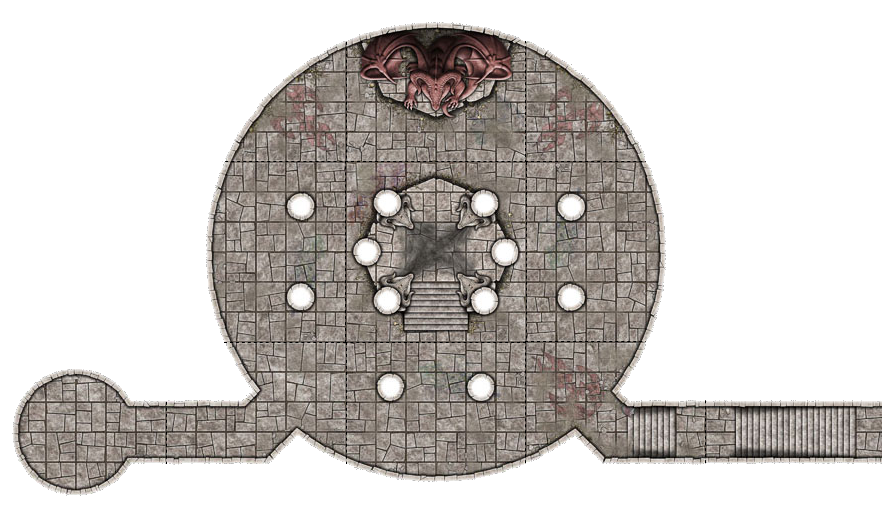
\includegraphics[width=7cm]{Maps/Temple.png}
\end{figure}

Le groupe se rend dans les quartiers où se trouvent le plus de démonistes. 
Alors qu'ils mènent leur enquête, ils sont guidé vers une auberge où se 
trouverait des cultistes. Alors que les joueurs sont dans l'auberge des sons 
étranges résonne dans le bâtiment. Le groupe est alors attaqué par un Vrock
(page \pageref{Vrock}). Lorsqu'ils trouvent le lieu d'origine de la bête, ils trouvent un 
pentacle de sang au sol et quelques cultistes qui se sont apparement saigné 
à mort pour l'invocation.

L'intérogatoire d'un survivant révèle que chaque meneur rassemble un petit 
cercle de fidèles et les dirigeants se regroupe dans une instance plus 
importante. Le groupe devra les infiltrer pour découvrir qui dirige réellement
le culte.

Prendre la place d'un meneur -> Diable à chaines.


Identifie le maitre démoniste

\subsection*{Le Club des Chasseurs}

Contact auprès de la guilde des alchimistes ou de la tour de magie


Identifie le maitre démoniste
